% Compile with LuaLaTeX
\documentclass[12pt,a4paper]{article}
\usepackage{fontspec}
\usepackage{polyglossia}
\setdefaultlanguage{ukrainian}
\setmainfont{NewComputerModern10}
\setsansfont{Noto Sans}
\setmonofont{Noto Sans Mono}[Scale=0.78]
\usepackage{amsmath,booktabs,caption,float,geometry,graphicx,microtype,titlesec,xcolor,array,tabularx,listings,needspace,enumitem}
\usepackage[
  unicode,
  colorlinks=true,
  linkcolor=black,
  urlcolor=blue,
  pdftitle={ІО-41, Давидчук Артем, Інформаційне забезпечення промислових роботів, Лабораторна робота №6},
  pdfauthor={Давидчук Артем},
  pdfsubject={Розподілена система керування робототехнічним комплексом}
]{hyperref}
\geometry{left=2cm,right=2cm,top=2cm,bottom=2cm}
\setlength{\parindent}{1.25cm}
\linespread{1.06}
\titleformat{\section}{\normalfont\fontsize{14}{16}\selectfont\bfseries}{\thesection}{0.6em}{}
\titlespacing*{\section}{0pt}{1.1em}{0.5em}
\captionsetup{font=small,labelfont=bf,labelsep=endash}
\renewcommand{\arraystretch}{1.17}
\newcolumntype{Y}{>{\raggedright\arraybackslash}X}
\definecolor{codebg}{RGB}{247,248,250}
\lstset{basicstyle=\ttfamily\scriptsize,breaklines=true,frame=single,
  backgroundcolor=\color{codebg},numbers=left,numberstyle=\tiny,
  xleftmargin=1.2em,framexleftmargin=1em,language=Python,
  showstringspaces=false,columns=fullflexible}
\setlist[itemize]{leftmargin=1.8em,itemsep=0.15em,topsep=0.25em}

\begin{document}
\pagenumbering{gobble}
\begin{titlepage}
  \begin{center}
\includegraphics[width=0.7\textwidth]{../../../../../templates/letterhead.png}\end{center}
  \begin{center}\large
    Національний технічний університет України\\
    «Київський політехнічний інститут імені Ігоря Сікорського»\\[1em]
    Факультет інформатики та обчислювальної техніки\\
    Кафедра обчислювальної техніки
  \end{center}
  \vfill
  \begin{center}
    \textbf{\LARGE Інформаційне забезпечення\\промислових роботів}\\[2em]
    \textbf{\Large Комп'ютерний практикум №6}\\[0.7em]
    \parbox{0.92\textwidth}{\centering
      «Розроблення розподіленої системи керування\\
      робототехнічним комплексом»}
  \end{center}
  \vfill
  \begin{flushright}\begin{minipage}{0.48\textwidth}
    Виконав: студент групи ІО-41\\
    \textit{Давидчук Артем}\\[1em]
    Перевірив: \textit{Тюляков Дмитро Ігорович}
  \end{minipage}\end{flushright}
  \vfill
  \begin{center}Київ --- 2026\end{center}
\end{titlepage}
\pagenumbering{arabic}

\section{Мета роботи}
Розробити розподілену систему керування робототехнічним комплексом,
у якій координатор взаємодіє з локальними контролерами окремих пристроїв.
Організувати обмін командами й станами, підтвердження прийняття та
виконання операцій, контроль зв'язку, журналювання і відновлення після
відмов.

\section{Постановка задачі}
За основу взято сортувальну комірку з лабораторних робіт №3 і №5:
конвеєр подає кольорову кульку, \texttt{Picker1} переносить її на стіл,
камера визначає колір, а \texttt{Picker2} кладе кульку у відповідний
контейнер. Сцену CoppeliaSim збережено у файлі \texttt{src/main.ttt}.

На відміну від лабораторної роботи №5, де один скінченний автомат
послідовно керував усією коміркою, у цій роботі керування розподілено:
координатор і чотири локальні контролери виконуються як окремі процеси.
Для відтворюваного тестування контролери обладнання реалізовано як тестові
моделі; їхні інтерфейси відповідають пристроям сцени CoppeliaSim.

\begin{figure}[H]
  \centering
  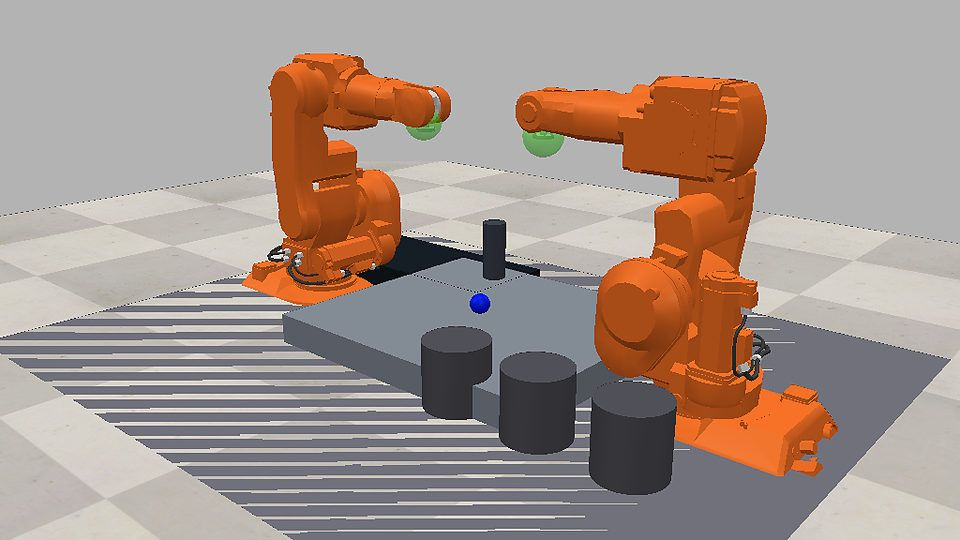
\includegraphics[width=0.73\textwidth]{scene_table.jpg}
  \caption{Загальний вигляд сортувальної комірки в CoppeliaSim}
  \label{fig:scene}
\end{figure}

\begin{figure}[H]
  \centering
  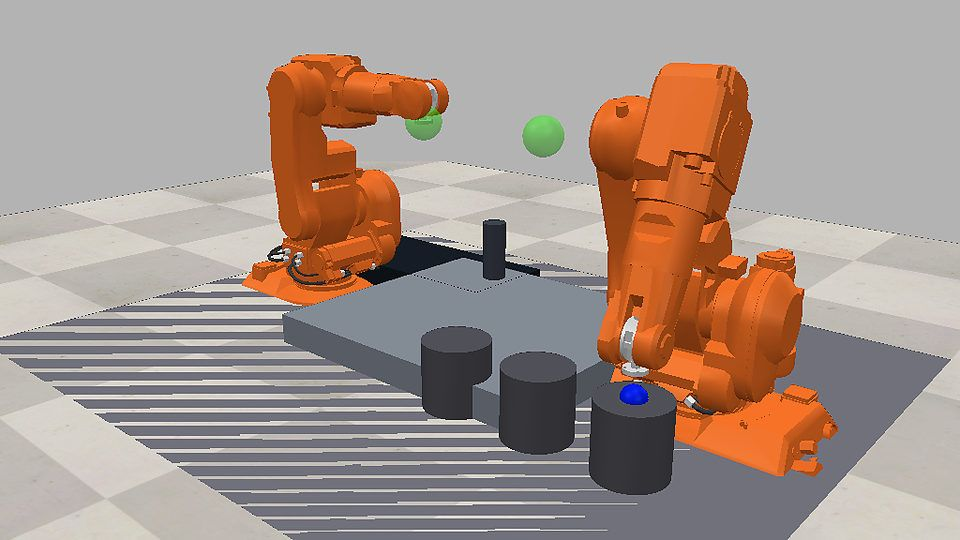
\includegraphics[width=0.73\textwidth]{scene_picker2.jpg}
  \caption{Сортування кульки маніпулятором \texttt{Picker2}}
  \label{fig:picker2}
\end{figure}

\section{Архітектура системи}
Координатор відкриває сокет типу \texttt{ROUTER}, а локальні контролери
підключаються до нього через сокети \texttt{DEALER}. Обмін виконується
через TCP за допомогою ZeroMQ; повідомлення кодуються у JSON. Така схема
дає змогу адресувати контролери за ідентифікатором та незалежно перевіряти
кожен компонент.

\begin{figure}[H]
  \centering
  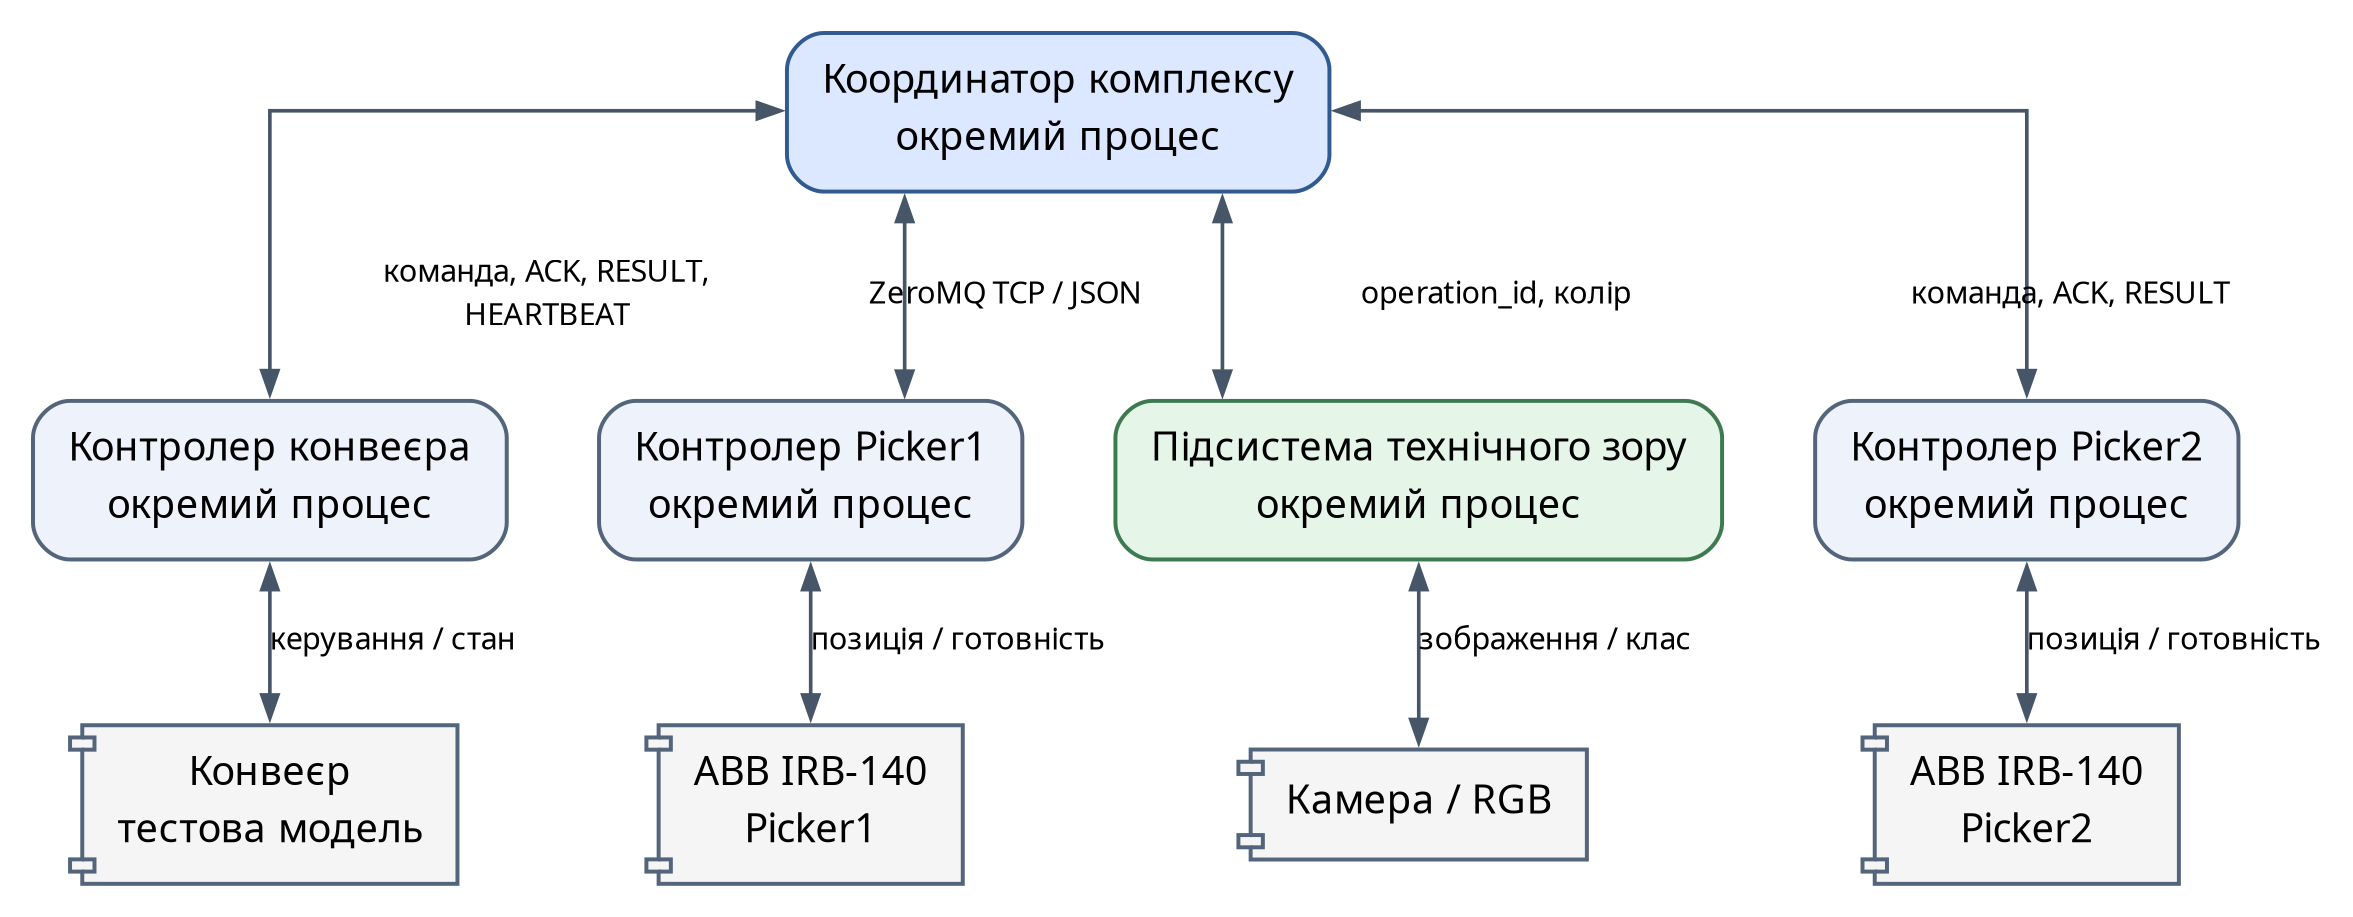
\includegraphics[width=\textwidth]{architecture.png}
  \caption{Структурна схема розподіленої системи керування}
  \label{fig:architecture}
\end{figure}

\begin{table}[H]
\centering\small\setlength{\tabcolsep}{5pt}
\begin{tabularx}{\textwidth}{@{}p{0.21\textwidth}YY@{}}
\toprule
\textbf{Компонент} & \textbf{Відповідальність} & \textbf{Основні команди та результати} \\
\midrule
Координатор & Формує послідовність операцій, контролює ACK, результат і тайм-аути & Надсилає команди, приймає \texttt{ACK}, \texttt{RESULT}, \texttt{HEARTBEAT} \\
Контролер конвеєра & Подає нову кульку до зони захоплення & \texttt{FEED\_BALL}, \texttt{RESET} \\
Контролер Picker1 & Переносить кульку з конвеєра на стіл & \texttt{MOVE\_TO\_TABLE}, \texttt{RESET} \\
Контролер зору & Визначає колір і достовірність результату & \texttt{CLASSIFY}; колір і \texttt{confidence} \\
Контролер Picker2 & Переносить кульку у вибраний контейнер & \texttt{SORT\_TO\_BIN}, \texttt{RESET} \\
\bottomrule
\end{tabularx}
\caption{Розподіл відповідальності між компонентами}
\label{tab:components}
\end{table}

\section{Стани та переходи}
Координатор очікує готовності всіх компонентів, а далі послідовно запускає
подавання, перенесення, розпізнавання і сортування. Помилка пристрою або
перевищення тайм-ауту переводить систему у \texttt{FAULT}; після
\texttt{RESET} виконується повторна перевірка готовності.

Локальний контролер приймає нову команду в стані \texttt{IDLE}, повертає
\texttt{ACK}, виконує дію в \texttt{BUSY} і надсилає \texttt{RESULT}.
Уже виконаний \texttt{operation\_id} зберігається: повтор тієї самої
команди повертає \texttt{DUPLICATE} без повторного руху механізму.

\begin{figure}[H]
  \centering
  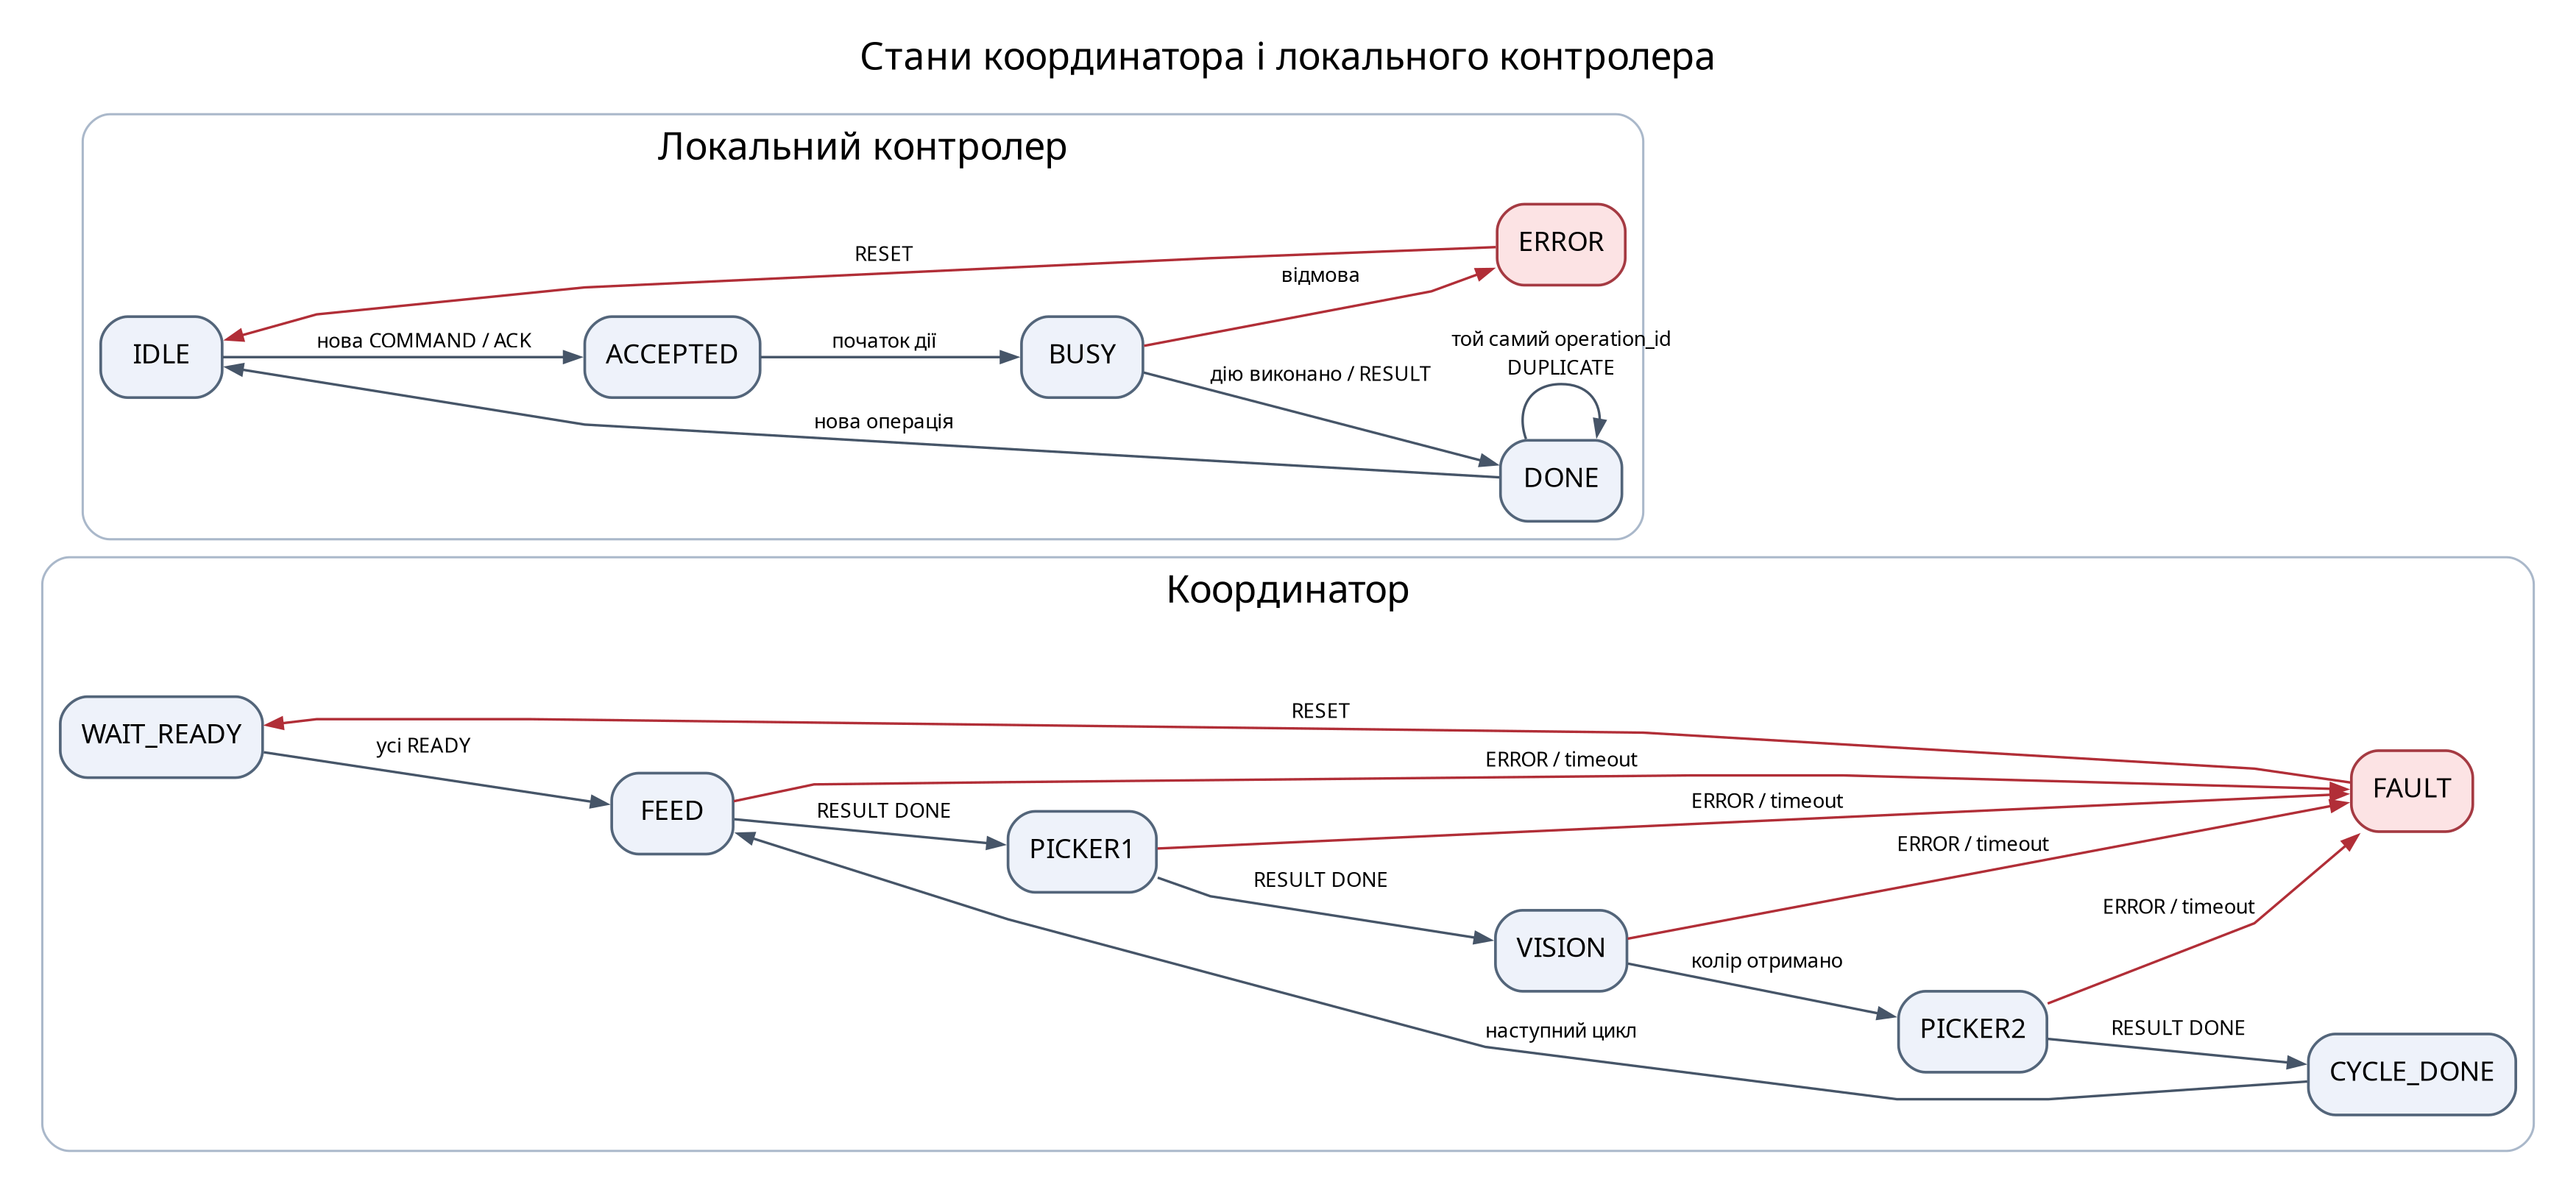
\includegraphics[width=\textwidth]{state_diagrams.png}
  \caption{Графи станів координатора та локального контролера}
  \label{fig:states}
\end{figure}

\begin{table}[H]
\centering\small\setlength{\tabcolsep}{4pt}
\begin{tabularx}{\textwidth}{@{}p{0.16\textwidth}p{0.27\textwidth}Yp{0.17\textwidth}@{}}
\toprule
\textbf{Стан} & \textbf{Подія або умова} & \textbf{Дія} & \textbf{Наступний стан} \\
\midrule
WAIT\_READY & Усі контролери надіслали \texttt{HELLO/READY} & Почати цикл & FEED \\
FEED & Конвеєр повернув \texttt{DONE} & Команда \texttt{MOVE\_TO\_TABLE} & PICKER1 \\
PICKER1 & Перенесення завершено & Команда \texttt{CLASSIFY} & VISION \\
VISION & Отримано колір & Передати колір у \texttt{SORT\_TO\_BIN} & PICKER2 \\
PICKER2 & Сортування завершено & Записати завершення циклу & CYCLE\_DONE \\
Штатний стан & \texttt{ERROR} або тайм-аут & Записати причину, припинити послідовність & FAULT \\
FAULT & Команда \texttt{RESET} & Скинути контролери & WAIT\_READY \\
\bottomrule
\end{tabularx}
\caption{Основні переходи координатора}
\label{tab:transitions}
\end{table}

\section{Сигнали, команди, події та таймери}
\textbf{Сигнали та повідомлення.} \texttt{HELLO/READY} сповіщає про запуск
контролера; \texttt{HEARTBEAT/ALIVE} підтверджує наявність зв'язку;
\texttt{ACK/ACCEPTED} означає прийняття операції; \texttt{RESULT} зі
статусом \texttt{DONE}, \texttt{ERROR} або \texttt{DUPLICATE} повідомляє
результат. Поле \texttt{payload} містить параметри або дані, наприклад
колір кульки та достовірність розпізнавання.

\textbf{Команди.} У штатному циклі застосовано \texttt{FEED\_BALL},
\texttt{MOVE\_TO\_TABLE}, \texttt{CLASSIFY} та
\texttt{SORT\_TO\_BIN}. Команда \texttt{RESET} відновлює компонент після
помилки. \texttt{PAUSE\_LINK} використовується лише в тесті втрати
зв'язку.

\textbf{Події.} Реєструються запуск контролерів, передавання команди,
отримання ACK і RESULT, завершення циклу, помилка пристрою, затримка ACK,
втрата та відновлення зв'язку, блокування дубліката і повторний запуск.
Кожний запис містить час, компонент, номер операції, категорію та опис.

\textbf{Таймери.} Контролери надсилають heartbeat кожні $0.20$~с.
Координатор очікує ACK не довше $0.50$~с, а результат --- не довше
$1.50$~с. У тесті затриманого підтвердження ACK навмисно затримано на
$0.45$~с при допустимих $0.15$~с. Втрата зв'язку моделюється паузою
$0.70$~с.

\section{Контракт обміну та промисловий протокол}
Кожне JSON-повідомлення містить поля \texttt{kind}, \texttt{component},
\texttt{operation\_id}, \texttt{command}, \texttt{status},
\texttt{payload} і \texttt{timestamp}. Унікальний номер операції дає
змогу зіставити ACK і RESULT з командою та забезпечити ідемпотентність.

Для ознайомчого відображення на промисловий протокол обрано Modbus TCP.
ZeroMQ використано в програмній моделі як транспорт між процесами, а
відповідні дані Modbus можуть бути розміщені так:

\begin{table}[H]
\centering\small
\begin{tabularx}{\textwidth}{@{}p{0.18\textwidth}p{0.22\textwidth}Y@{}}
\toprule
\textbf{Адреса} & \textbf{Дані} & \textbf{Призначення} \\
\midrule
Coil 00001 & START / RESET & Запуск або скидання локального контролера \\
HR 40001 & Код команди & FEED, MOVE, CLASSIFY, SORT або RESET \\
HR 40002--40003 & \texttt{operation\_id} & Старше і молодше слово номера операції \\
HR 40004 & Параметр & Код кольору або параметр команди \\
IR 30001 & Стан & IDLE, ACCEPTED, BUSY, DONE чи ERROR \\
IR 30002 & Статус & ACK, DONE, ERROR або DUPLICATE \\
IR 30003 & Код помилки & Нуль або код відмови пристрою \\
IR 30004 & Heartbeat & Лічильник активності контролера \\
\bottomrule
\end{tabularx}
\caption{Запропонована карта регістрів Modbus TCP}
\label{tab:modbus}
\end{table}

\section{Фрагменти програми}
Метод \texttt{execute} надсилає команду, окремо контролює час очікування
ACK і RESULT та відкидає повідомлення з іншим номером операції.

\lstinputlisting[firstline=104,lastline=135,caption={Обмін командою та контроль тайм-аутів},label={lst:execute}]{../src/main.py}

Штатний цикл утворюється послідовністю чотирьох адресних команд. Результат
камери передається контролеру другого маніпулятора як параметр.

\lstinputlisting[firstline=137,lastline=146,caption={Послідовність одного циклу сортування},label={lst:cycle}]{../src/main.py}

Локальний контролер зберігає результати завершених операцій. Якщо команда
з тим самим \texttt{operation\_id} надходить повторно, фізична дія не
запускається.

\lstinputlisting[firstline=116,lastline=139,caption={Ідемпотентна обробка команди локальним контролером},label={lst:duplicate}]{../src/controller.py}

\section{Інтеграційне тестування}
Запущено три штатні цикли, після чого автоматично виконано всі передбачені
аварійні сценарії. Після скидання проведено ще один повний цикл.

\begin{table}[H]
\centering\small\setlength{\tabcolsep}{4pt}
\begin{tabularx}{\textwidth}{@{}p{0.23\textwidth}Yp{0.17\textwidth}@{}}
\toprule
\textbf{Тест} & \textbf{Очікувана реакція} & \textbf{Результат} \\
\midrule
Штатний цикл & Чотири операції завершуються \texttt{DONE}, колір передано Picker2 & Пройдено \\
Відмова пристрою & Picker2 повертає \texttt{ERROR}; помилку зафіксовано & Пройдено \\
Втрата зв'язку & Виникає тайм-аут ACK; після \texttt{RESET} зв'язок відновлено & Пройдено \\
Затриманий ACK & Координатор фіксує перевищення тайм-ауту & Пройдено \\
Повтор команди & Другий запит має статус \texttt{DUPLICATE} і не виконується & Пройдено \\
Скидання і перезапуск & Усі компоненти скинуто, новий цикл завершено & Пройдено \\
\bottomrule
\end{tabularx}
\caption{Результати інтеграційних тестів}
\label{tab:tests}
\end{table}

\begin{lstlisting}[caption={Фрагмент журналу тестування}]
1.67 | picker2     | op-0013      | RESULT   | ERROR
2.17 | coordinator | link-test    | TIMEOUT  | conveyor ACK timeout
3.20 | coordinator | delay-test   | TIMEOUT  | picker1 ACK timeout
3.82 | vision      | duplicate-001| RESULT   | DUPLICATE
4.79 | coordinator | cycle-4      | CYCLE    | completed; colour=red
\end{lstlisting}

Підсумок програми: виконано чотири повні цикли; тести відмови пристрою,
втрати зв'язку, затриманого ACK, дубліката та перезапуску завершилися
успішно.

\section{Запуск}
У каталозі \texttt{lab6} виконати:
\begin{lstlisting}[numbers=none,language={}]
python src/main.py --cycles 3
python src/test_distributed.py
\end{lstlisting}
Перший виклик запускає демонстрацію та створює
\texttt{logs/integration.log}; другий запускає повторювані автоматичні
перевірки. Для перегляду початкової робототехнічної комірки слід відкрити
\texttt{src/main.ttt} у CoppeliaSim.

\section{Висновки}
У роботі централізований автомат сортувальної комірки перетворено на
ієрархічну розподілену систему: координатор визначає послідовність, а
локальні контролери відповідають за окремі пристрої. Порівняно з єдиним
контролером така структура складніша через мережеві тайм-аути та потребу
ідентифікувати операції, проте вона краще локалізує відмови й дозволяє
незалежно масштабувати компоненти. ACK/RESULT, heartbeat,
\texttt{operation\_id}, журналювання та команда RESET забезпечили
контрольоване відновлення після всіх перевірених аварій.

\end{document}
